%! TEX program = xelatex
%! TEX root = ../root.tex

\section{实验原理}
\subsection{Datapath}
为了支持多周期操作本实验对数据通路进行了修改,想要成功完成此次实验,对Datapath的熟练掌握自然是必要的。
下面就是本次实验所参照的Datapath

\begin{figure}[H] %H为当前位置,!htb为忽略美学标准,htbp为浮动图形
	\centering %图片居中
	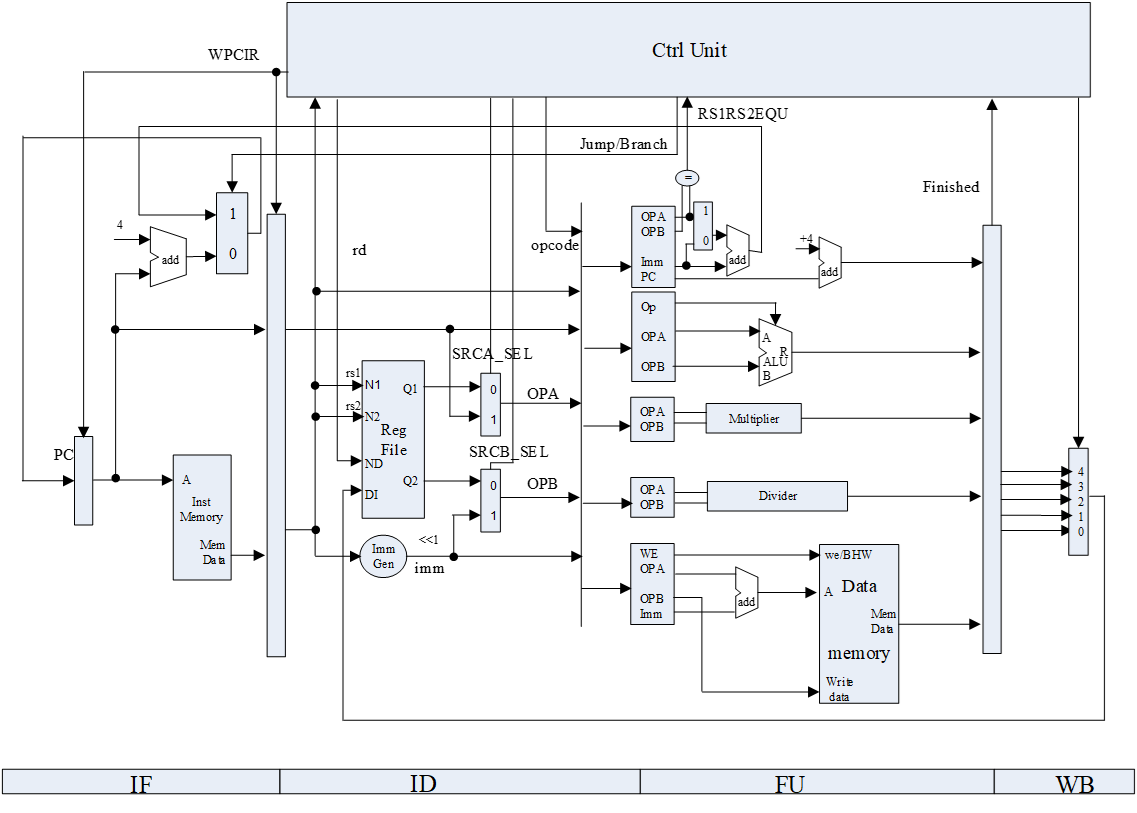
\includegraphics[width=1.0\textwidth]{figs/DataPath.png} %插入图片,[]中设置图片大小,{}中是图片文件名
	\caption{Datapath} %最终文档中希望显示的图片标题
	\label{Fig.1} %用于文内引用的标签
\end{figure}

根据此图,我们就能够将数据通路部分完成,完成的RV32Core.v代码如下所示:
\begin{lstlisting}[language = {verilog}]
`timescale 1ns / 1ps

module  RV32core(
		input debug_en,  // debug enable
		input debug_step,  // debug step clock
		input [6:0] debug_addr,  // debug address
		output[31:0] debug_data,  // debug data
		input clk,  // main clock
		input rst,  // synchronous reset
		input interrupter  // interrupt source, for future use
	);

	wire debug_clk;
	wire[31:0] debug_regs;
	reg[31:0] Test_signal;
	assign debug_data = debug_addr[5] ? Test_signal : debug_regs;

	debug_clk clock(.clk(clk),.debug_en(debug_en),.debug_step(debug_step),.debug_clk(debug_clk));

	wire reg_IF_EN, reg_ID_EN, reg_ID_flush, FU_ALU_EN, FU_mem_EN, FU_mul_EN, FU_div_EN, FU_jump_EN;
	wire RegWrite_ctrl, ALUSrcA_ctrl, ALUSrcB_ctrl, mem_w_ctrl, branch_ctrl;
	wire[2:0] ImmSel_ctrl, DatatoReg_ctrl;
	wire[3:0] ALUControl_ctrl, Jump_ctrl;
	wire[4:0] rd_ctrl;


	wire [31:0] PC_IF, next_PC_IF, PC_4_IF, inst_IF;

	wire valid_ID;
	wire[31:0]inst_ID, PC_ID, Imm_out_ID, rs1_data_ID, rs2_data_ID, ALUA_ID, ALUB_ID;

	wire FU_ALU_finish, FU_mem_finish, FU_mul_finish, FU_div_finish, FU_jump_finish, cmp_res_FU;
	wire[31:0]ALUout_FU, mem_data_FU, mulres_FU, divres_FU, PC_jump_FU, PC_wb_FU;

	wire[31:0]ALUout_WB, mem_data_WB, mulres_WB, divres_WB, PC_wb_WB, wt_data_WB;


	// IF
	REG32 REG_PC(.clk(debug_clk),.rst(rst),.CE(reg_IF_EN),.D(next_PC_IF),.Q(PC_IF));
	
	add_32 add_IF(.a(PC_IF),.b(32'd4),.c(PC_4_IF));

	MUX2T1_32 mux_IF(.I0(PC_4_IF),.I1(PC_jump_FU),.s(branch_ctrl),.o(next_PC_IF));

	ROM_D inst_rom(.a(PC_IF[8:2]),.spo(inst_IF));


	//Issue
	REG_ID reg_ID(.clk(debug_clk),.rst(rst),.EN(reg_ID_EN),
		.flush(reg_ID_flush),.PCOUT(PC_IF),.IR(inst_IF),

		.IR_ID(inst_ID),.PCurrent_ID(PC_ID),.valid(valid_ID));
	
	CtrlUnit ctrl(.clk(debug_clk),.rst(rst),.inst(inst_ID),.valid_ID(valid_ID),
		.ALU_done(FU_ALU_finish),.MEM_done(FU_mem_finish),.MUL_done(FU_mul_finish),
		.DIV_done(FU_div_finish),.JUMP_done(FU_jump_finish),.cmp_res_FU(cmp_res_FU),

		.reg_IF_en(reg_IF_EN),.branch_ctrl(branch_ctrl),.reg_ID_en(reg_ID_EN),
		.reg_ID_flush(reg_ID_flush),.ImmSel(ImmSel_ctrl),.ALU_en(FU_ALU_EN),
		.MEM_en(FU_mem_EN),.MUL_en(FU_mul_EN),.DIV_en(FU_div_EN),.JUMP_en(FU_jump_EN),
		.JUMP_op(Jump_ctrl),.ALU_op(ALUControl_ctrl),.MEM_we(mem_w_ctrl),
		.ALUSrcA(ALUSrcA_ctrl),.ALUSrcB(ALUSrcB_ctrl),
		.write_sel(DatatoReg_ctrl),.reg_write(RegWrite_ctrl),.rd_ctrl(rd_ctrl));

	ImmGen imm_gen(.ImmSel(ImmSel_ctrl), .inst_field(inst_ID), .Imm_out(Imm_out_ID));            //to fill sth.in

	Regs register(.clk(debug_clk),.rst(rst),
		.R_addr_A(inst_ID[19:15]),.rdata_A(rs1_data_ID),
		.R_addr_B(inst_ID[24:20]),.rdata_B(rs2_data_ID),
		.L_S(RegWrite_ctrl),.Wt_addr(rd_ctrl),.Wt_data(wt_data_WB),
		.Debug_addr(debug_addr[4:0]),.Debug_regs(debug_regs));

	MUX2T1_32 mux_imm_ALU_ID_A(.I0(rs1_data_ID), .I1(PC_ID), .s(ALUSrcA_ctrl), .o(ALUA_ID));            //to fill sth.in

	MUX2T1_32 mux_imm_ALU_ID_B(.I0(rs2_data_ID), .I1(PC_ID), .s(ALUSrcB_ctrl), .o(ALUB_ID));            //to fill sth.in


	// FU
	FU_ALU alu(.clk(debug_clk),.EN(FU_ALU_EN),.finish(FU_ALU_finish),
		.ALUControl(ALUControl_ctrl),.ALUA(ALUA_ID),.ALUB(ALUB_ID),.res(ALUout_FU),
		.zero(),.overflow());

	FU_mem mem(.clk(debug_clk),.EN(FU_mem_EN),.finish(FU_mem_finish),
		.mem_w(mem_w_ctrl),.bhw(inst_ID[14:12]),.rs1_data(rs1_data_ID),.rs2_data(rs2_data_ID),
		.imm(Imm_out_ID),.mem_data(mem_data_FU));

	FU_mul mu(.clk(debug_clk),.EN(FU_mul_EN),.finish(FU_mul_finish),
		.A(rs1_data_ID),.B(rs2_data_ID),.res(mulres_FU));

	FU_div du(.clk(debug_clk),.EN(FU_div_EN),.finish(FU_div_finish),
		.A(rs1_data_ID),.B(rs2_data_ID),.res(divres_FU));

	FU_jump ju(.clk(debug_clk),.EN(FU_jump_EN),.finish(FU_jump_finish),
		.JALR(Jump_ctrl[3]),.cmp_ctrl(Jump_ctrl[2:0]),.rs1_data(rs1_data_ID),.rs2_data(rs2_data_ID),
		.imm(Imm_out_ID),.PC(PC_ID),.PC_jump(PC_jump_FU),.PC_wb(PC_wb_FU),.cmp_res(cmp_res_FU));


	// WB
	REG32 reg_WB_ALU(.clk(debug_clk),.rst(rst),.CE(FU_ALU_finish),.D(ALUout_FU),.Q(ALUout_WB));

	REG32 reg_WB_mem(.clk(debug_clk),.rst(rst),.CE(FU_mem_finish),.D(mem_data_FU),.Q(mem_data_WB));

	REG32 reg_WB_mul(.clk(debug_clk),.rst(rst),.CE(FU_mul_finish),.D(mulres_FU),.Q(mulres_WB));

	REG32 reg_WB_div(.clk(debug_clk),.rst(rst),.CE(FU_div_finish),.D(divres_FU),.Q(divres_WB));
	
	REG32 reg_WB_jump(.clk(debug_clk),.rst(rst),.CE(FU_jump_finish),.D(PC_wb_FU),.Q(PC_wb_WB));

	MUX8T1_32 mux_DtR(.s(DatatoReg_ctrl), .I0(32'd0), .I1(ALUout_WB), .I2(mem_data_WB), .I3(mulres_WB),
	.I4(divres_WB), .I5(PC_wb_WB), .I6(32'd0), .I7(32'd0), .o(wt_data_WB));  //to fill sth.in


	always @* begin
		case (debug_addr[4:0])
			0:  Test_signal = PC_IF;
			1:  Test_signal = inst_IF;
			2:  Test_signal = PC_ID;  
			3:  Test_signal = inst_ID;

			4:  Test_signal = inst_ID[19:15];
			5:  Test_signal = rs1_data_ID;
			6:  Test_signal = inst_ID[24:20];
			7:  Test_signal = rs2_data_ID;

			8:  Test_signal = ImmSel_ctrl;
			9:  Test_signal = Imm_out_ID;
			10: Test_signal = ALUout_FU;
			11: Test_signal = reg_IF_EN;

			12: Test_signal = {15'b0, FU_ALU_EN, 15'b0, FU_ALU_finish};
			13: Test_signal = ALUControl_ctrl;
			14: Test_signal = ALUA_ID;
			15: Test_signal = ALUB_ID;

			16: Test_signal = {15'b0, FU_mem_EN, 15'b0, FU_mem_finish};
			17: Test_signal = mem_w_ctrl;
			18: Test_signal = inst_ID[14:12];
			19: Test_signal = mem_data_FU;

			20: Test_signal = {15'b0, FU_mul_EN, 15'b0, FU_mul_finish};
			21: Test_signal = mulres_FU;
			22: Test_signal = {15'b0, FU_div_EN, 15'b0, FU_div_finish};
			23: Test_signal = divres_FU;

			24: Test_signal = {15'b0, FU_jump_EN, 15'b0, FU_jump_finish};
			25: Test_signal = Jump_ctrl;
			26: Test_signal = PC_jump_FU;
			27: Test_signal = PC_wb_FU;

			28: Test_signal = RegWrite_ctrl;
			29: Test_signal = rd_ctrl;
			30: Test_signal = DatatoReg_ctrl;
			31: Test_signal = wt_data_WB;
			
			default: Test_signal = 32'hAA55_AA55;
		endcase
	end

endmodule
\end{lstlisting}

\subsection{Data Hazard}
但流水线支持多周期操作后,势必会更改Data Hazard的情形和解决方式,为了解决这一问题,
此实验中简单的使用了FU阶段的各操作的finish信号进行Data Hazard的resolve,只有当一条指令的FU阶段结束之后才允许
进入WB阶段,当然仅仅只控制当前执行指令停顿是远远不够的,此次实验中还将FU的结束信号传入了Ctrl Unit中,作为Data Hazard的检测信号,
当FU阶段未结束时,Ctrl Unit中的FU_in_use信号会升起,并且会使得后续指令同样等待FU阶段结束。\\
具体例子如下所示:

\begin{figure}[H] %H为当前位置,!htb为忽略美学标准,htbp为浮动图形
	\centering %图片居中
	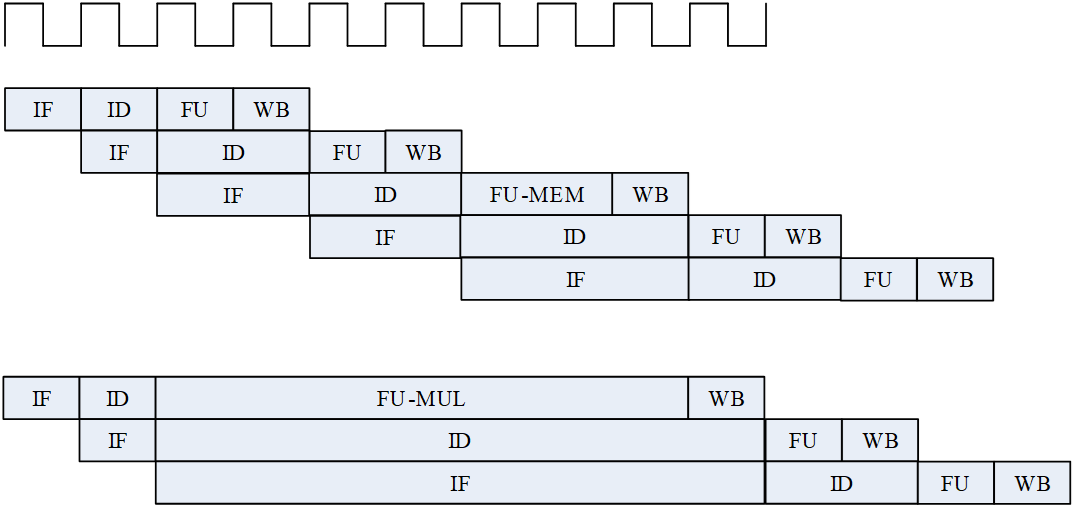
\includegraphics[width=1.0\textwidth]{figs/DataHazard.png} %插入图片,[]中设置图片大小,{}中是图片文件名
	\caption{DataHazard} %最终文档中希望显示的图片标题
	\label{Fig.2} %用于文内引用的标签
\end{figure}
当CPU需要对数据进行操作时,会首先传入read或write bit。CMU接收到信号后首先查看地址是否hit,若hit则直接读或写数据。否则检查需要置换的block是否dirty,若dirty则需要先将当前块写回memory。之后从memory中取数据存入cache,再进行读或写操作。
\subsection{Cache Management State Machine}
CMU的内部结构实际上是一个有限状态机,其有S\_IDLE、S\_PRE\_BACK、S\_BACK、S\_FILL、S\_WAIT等5个状态。
\begin{figure}[H] %H为当前位置,!htb为忽略美学标准,htbp为浮动图形
	\centering %图片居中
	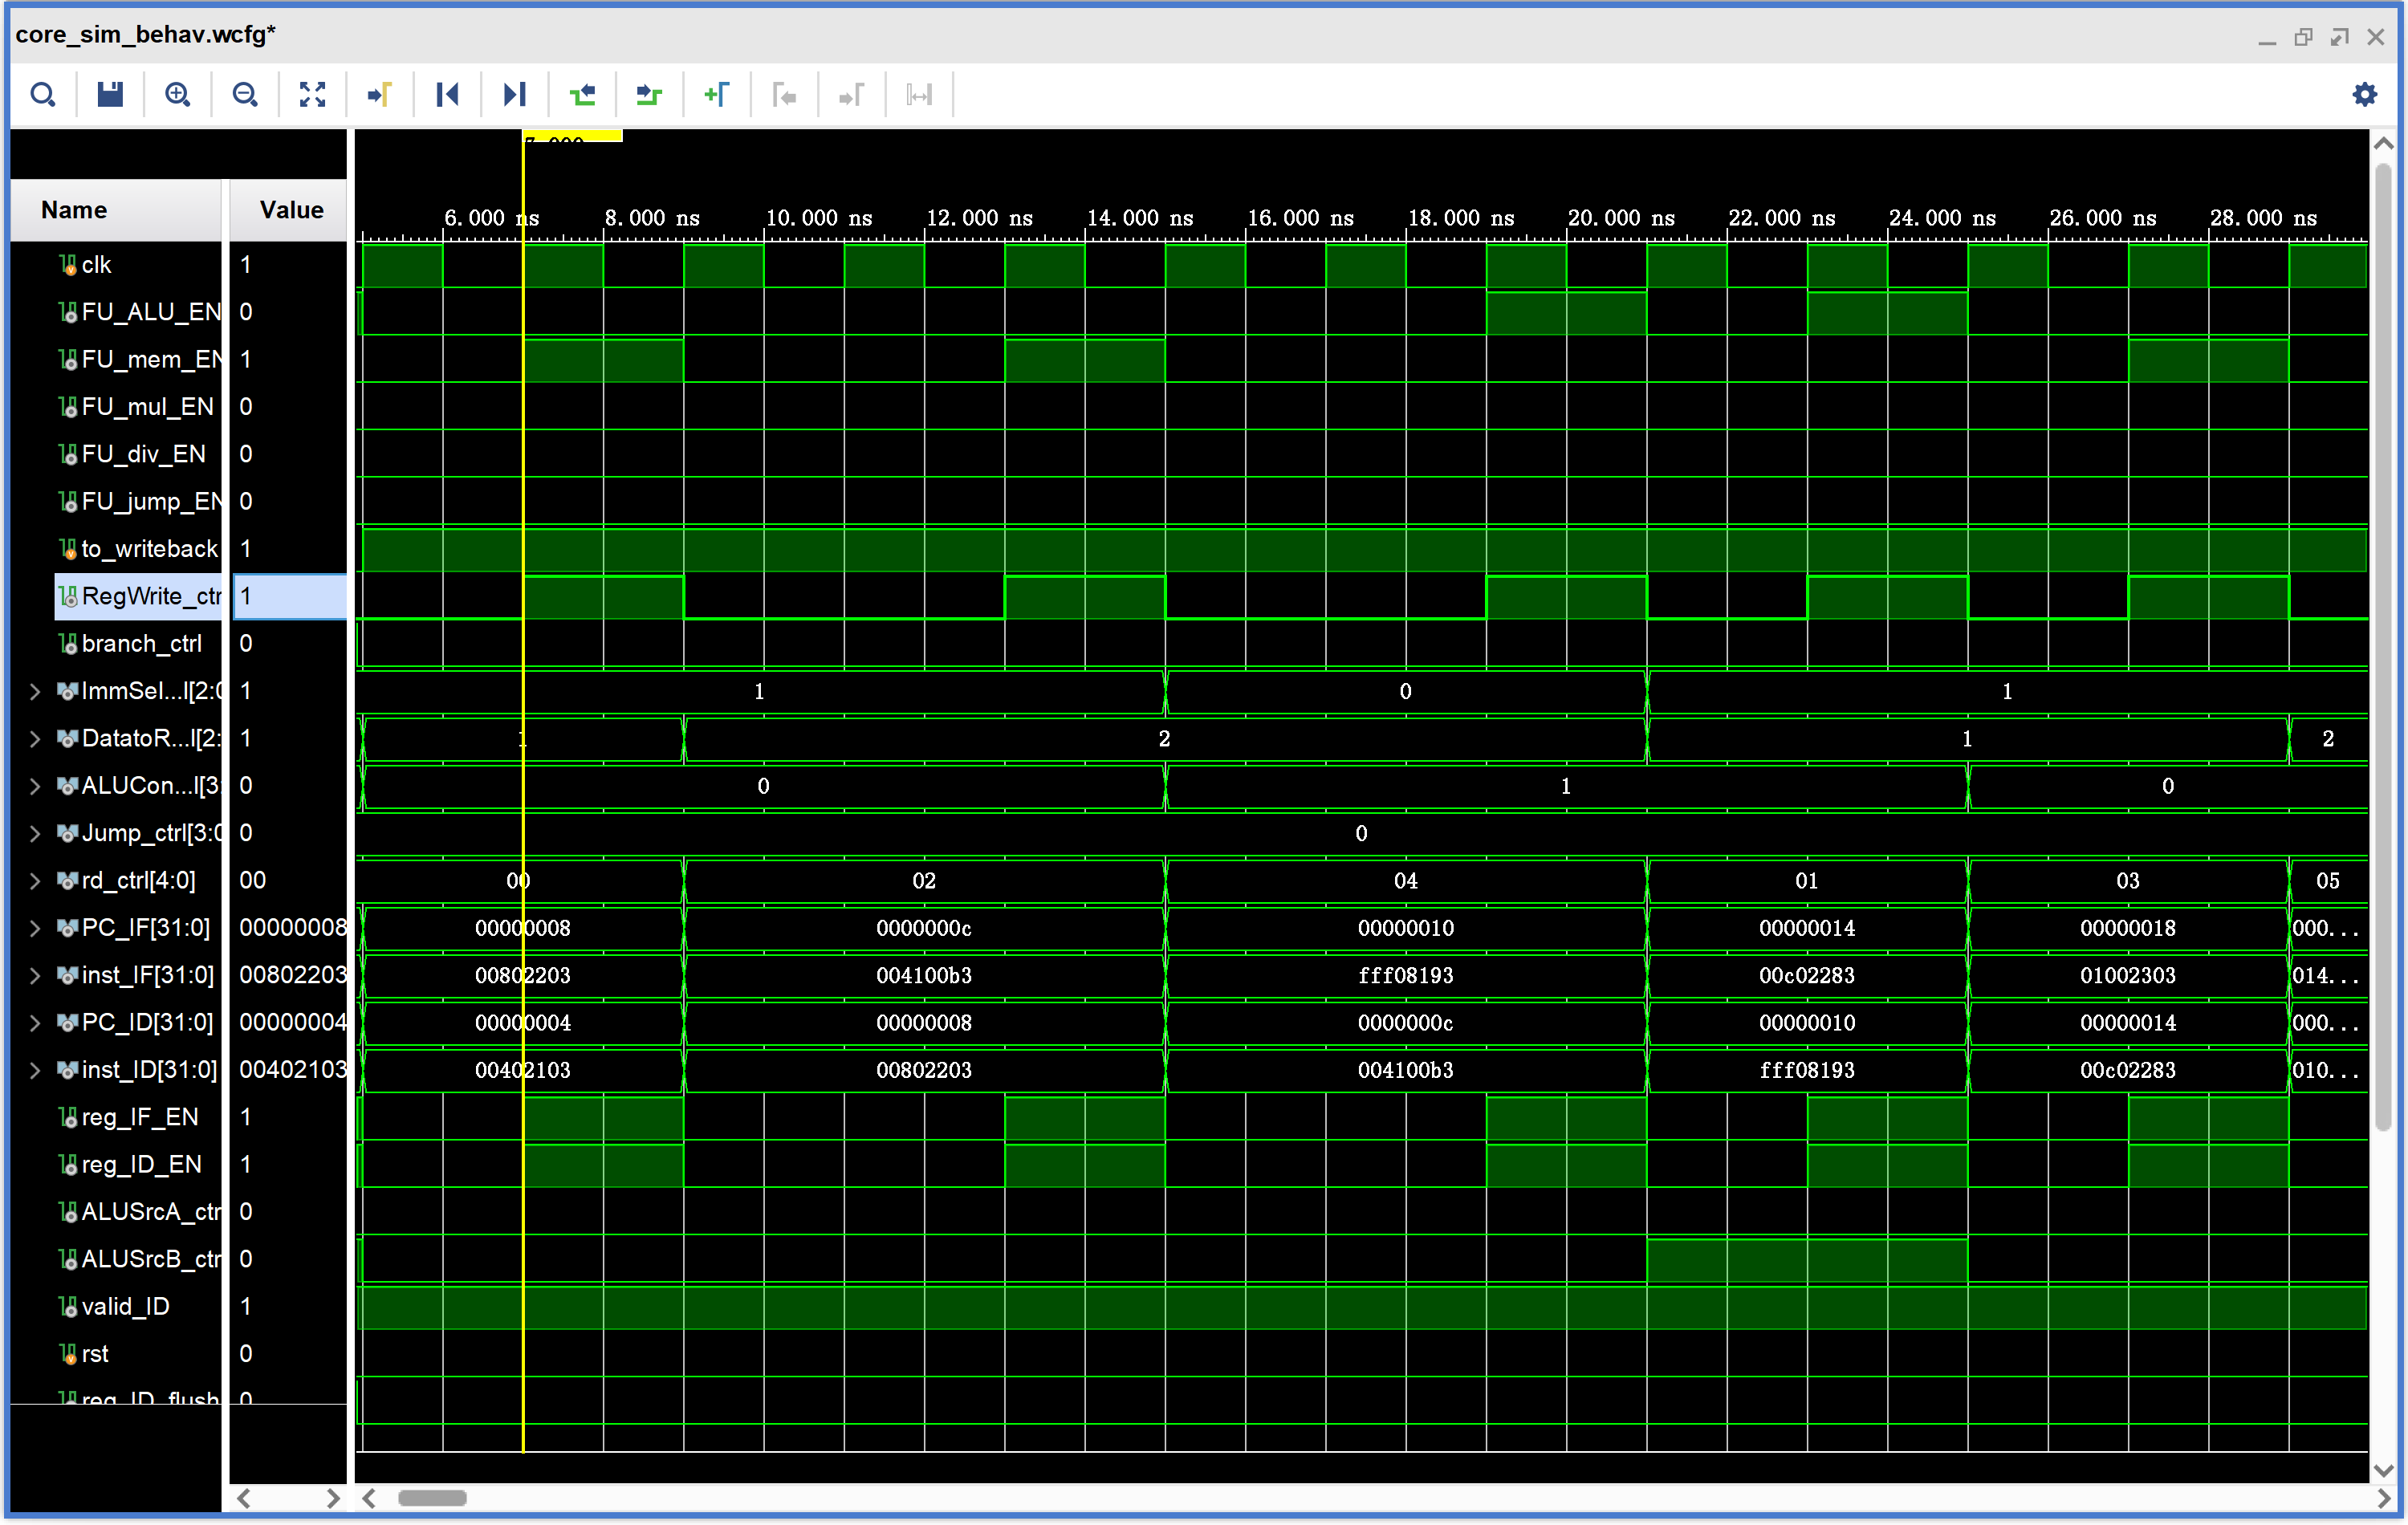
\includegraphics[width=1.0\textwidth]{figs/2.png} %插入图片,[]中设置图片大小,{}中是图片文件名
	\caption{CMU状态机} %最终文档中希望显示的图片标题
	\label{Fig.3} %用于文内引用的标签
\end{figure}
cache操作均发生在当前state的下降沿,memory操作均发生在当前state的上升沿。 每个状态的具体描述如下:
\begin{itemize}
	\item [1.] S\_IDLE:空闲状态,不进行memory操作,cache操作hit的情况下一直处于这个状态。
	\item [2.] S\_PRE\_BACK:为了写回,先进行一次读cache。
	\item [3.] S\_BACK:上升沿将上个状态的数据写回到memory,下降沿从cache读下次需要写回的数据,由计数器控制直到整个cache line全部写回。由于memory设置为4个周期完成读写操作,因此需要等待memory给出ack信号,才能进行状态的改变。
	\item [4.] S\_FILL:上升沿从memory读取数据,下降沿向cache写入数据,由计数器控制直到整个cache line全部写入。与S\_BACK类似,需要等待ack信号。
	\item [5.] S\_WAIT:执行之前由于miss而不能进行的cache操作。
\end{itemize}
\subsection{源代码}
\begin{lstlisting}[language = {verilog}]
module cmu (
	// CPU side
	input clk,
	input rst,
	input [31:0] addr_rw,
	input en_r,
	input en_w,
	input [2:0] u_b_h_w,
	input [31:0] data_w,
	output [31:0] data_r,
	output stall,
	
	// mem side
	output reg mem_cs_o = 0,
	output reg mem_we_o = 0,
	output reg [31:0] mem_addr_o = 0,
	input [31:0] mem_data_i,
	output [31:0] mem_data_o,
	input mem_ack_i,
	
	// debug info
	output [2:0] cmu_state
	);
	
	`include "addr_define.vh"
	
	reg [ADDR_BITS-1:0] cache_addr = 0;
	reg cache_load = 0;
	reg cache_store = 0;
	reg cache_edit = 0;
	reg [2:0] cache_u_b_h_w = 0;
	reg [WORD_BITS-1:0] cache_din = 0;
	wire cache_hit;
	wire [WORD_BITS-1:0] cache_dout;
	wire cache_valid;
	wire cache_dirty;
	wire [TAG_BITS-1:0] cache_tag;
	
	cache CACHE (
	.clk(~clk),
	.rst(rst),
	.addr(cache_addr),
	.load(cache_load),
	.store(cache_store),
	.edit(cache_edit),
	.invalid(1'b0),
	.u_b_h_w(cache_u_b_h_w),
	.din(cache_din),
	.hit(cache_hit),
	.dout(cache_dout),
	.valid(cache_valid),
	.dirty(cache_dirty),
	.tag(cache_tag)
	);
	
	localparam
	S_IDLE = 0,
	S_PRE_BACK = 1,
	S_BACK = 2,
	S_FILL = 3,
	S_WAIT = 4;
	
	reg [2:0]state = 0;
	reg [2:0]next_state = 0;
	reg [ELEMENT_WORDS_WIDTH-1:0]word_count = 0;
	reg [ELEMENT_WORDS_WIDTH-1:0]next_word_count = 0;
	assign cmu_state = state;
	
	always @ (posedge clk) begin
	if (rst) begin
	state <= S_IDLE;
	word_count <= 2'b00;
	end
	else begin
	state <= next_state;
	word_count <= next_word_count;
	end
	end
	
	// state ctrl
	always @ (*) begin
	if (rst) begin
	next_state = S_IDLE;
	next_word_count = 2'b00;
	end
	else begin
	case (state)
	S_IDLE: begin
	if (en_r || en_w) begin
	if (cache_hit)
	next_state = S_IDLE;
	else if (cache_valid && cache_dirty)
	next_state = S_PRE_BACK;
	else
	next_state = S_FILL;
	end
	next_word_count = 2'b00;
	end
	
	S_PRE_BACK: begin
	next_state = S_BACK;
	next_word_count = 2'b00;
	end
	
	S_BACK: begin //?
	if (mem_ack_i && word_count == {ELEMENT_WORDS_WIDTH{1'b1}})    // 2'b11 in default case
	next_state = S_FILL;
	else
	next_state = S_BACK;
	
	if (mem_ack_i)
	next_word_count = word_count + 2'b01; //?
	else
	next_word_count = word_count;
	end
	
	S_FILL: begin
	if (mem_ack_i && word_count == {ELEMENT_WORDS_WIDTH{1'b1}})
	next_state = S_WAIT;
	else
	next_state = S_FILL;
	
	if (mem_ack_i)
	next_word_count = word_count + 2'b01;
	else
	next_word_count = word_count;
	end
	
	S_WAIT: begin
	next_state = S_IDLE;
	next_word_count = 2'b00;
	end
	endcase
	end
	end
	
	// cache ctrl
	always @ (*) begin
	case(state)
	S_IDLE, S_WAIT: begin
	cache_addr = addr_rw;
	cache_load = en_r;
	cache_edit = en_w;
	cache_store = 1'b0;
	cache_u_b_h_w = u_b_h_w;
	cache_din = data_w;
	end
	S_BACK, S_PRE_BACK: begin
	cache_addr = {addr_rw[ADDR_BITS-1:BLOCK_WIDTH], next_word_count, {ELEMENT_WORDS_WIDTH{1'b0}}};
	cache_load = 1'b0;
	cache_edit = 1'b0;
	cache_store = 1'b0;
	cache_u_b_h_w = 3'b010;
	cache_din = 32'b0;
	end
	S_FILL: begin
	cache_addr = {addr_rw[ADDR_BITS-1:BLOCK_WIDTH], word_count, {ELEMENT_WORDS_WIDTH{1'b0}}};
	cache_load = 1'b0;
	cache_edit = 1'b0;
	cache_store = mem_ack_i;
	cache_u_b_h_w = 3'b010;
	cache_din = mem_data_i;
	end
	endcase
	end
	assign data_r = cache_dout;
	
	// mem ctrl
	always @ (*) begin
	case (next_state)
	S_IDLE, S_PRE_BACK, S_WAIT: begin
	mem_cs_o = 1'b0;
	mem_we_o = 1'b0;
	mem_addr_o = 32'b0;
	end
	
	S_BACK: begin
	mem_cs_o = 1'b1;
	mem_we_o = 1'b1;
	mem_addr_o = {cache_tag, addr_rw[ADDR_BITS-TAG_BITS-1:BLOCK_WIDTH], next_word_count, {ELEMENT_WORDS_WIDTH{1'b0}}};
	end
	
	S_FILL: begin
	mem_cs_o = 1'b1;
	mem_we_o = 1'b0;
	mem_addr_o = {addr_rw[ADDR_BITS-1:BLOCK_WIDTH], next_word_count, {ELEMENT_WORDS_WIDTH{1'b0}}};
	end
	endcase
	end
	assign mem_data_o = cache_dout;
	
	//important
	assign stall = (next_state != S_IDLE);
	
endmodule
	
\end{lstlisting}